\documentclass[]{article}
\usepackage{lmodern}
\usepackage{amssymb,amsmath}
\usepackage{ifxetex,ifluatex}
\usepackage{fixltx2e} % provides \textsubscript
\ifnum 0\ifxetex 1\fi\ifluatex 1\fi=0 % if pdftex
  \usepackage[T1]{fontenc}
  \usepackage[utf8]{inputenc}
\else % if luatex or xelatex
  \ifxetex
    \usepackage{mathspec}
  \else
    \usepackage{fontspec}
  \fi
  \defaultfontfeatures{Ligatures=TeX,Scale=MatchLowercase}
\fi
% use upquote if available, for straight quotes in verbatim environments
\IfFileExists{upquote.sty}{\usepackage{upquote}}{}
% use microtype if available
\IfFileExists{microtype.sty}{%
\usepackage{microtype}
\UseMicrotypeSet[protrusion]{basicmath} % disable protrusion for tt fonts
}{}
\usepackage[margin=1in]{geometry}
\usepackage{hyperref}
\hypersetup{unicode=true,
            pdftitle={SoftMax Weights for a Weighted Least Squares Linear Model},
            pdfauthor={R-team},
            pdfborder={0 0 0},
            breaklinks=true}
\urlstyle{same}  % don't use monospace font for urls
\usepackage{color}
\usepackage{fancyvrb}
\newcommand{\VerbBar}{|}
\newcommand{\VERB}{\Verb[commandchars=\\\{\}]}
\DefineVerbatimEnvironment{Highlighting}{Verbatim}{commandchars=\\\{\}}
% Add ',fontsize=\small' for more characters per line
\usepackage{framed}
\definecolor{shadecolor}{RGB}{248,248,248}
\newenvironment{Shaded}{\begin{snugshade}}{\end{snugshade}}
\newcommand{\KeywordTok}[1]{\textcolor[rgb]{0.13,0.29,0.53}{\textbf{#1}}}
\newcommand{\DataTypeTok}[1]{\textcolor[rgb]{0.13,0.29,0.53}{#1}}
\newcommand{\DecValTok}[1]{\textcolor[rgb]{0.00,0.00,0.81}{#1}}
\newcommand{\BaseNTok}[1]{\textcolor[rgb]{0.00,0.00,0.81}{#1}}
\newcommand{\FloatTok}[1]{\textcolor[rgb]{0.00,0.00,0.81}{#1}}
\newcommand{\ConstantTok}[1]{\textcolor[rgb]{0.00,0.00,0.00}{#1}}
\newcommand{\CharTok}[1]{\textcolor[rgb]{0.31,0.60,0.02}{#1}}
\newcommand{\SpecialCharTok}[1]{\textcolor[rgb]{0.00,0.00,0.00}{#1}}
\newcommand{\StringTok}[1]{\textcolor[rgb]{0.31,0.60,0.02}{#1}}
\newcommand{\VerbatimStringTok}[1]{\textcolor[rgb]{0.31,0.60,0.02}{#1}}
\newcommand{\SpecialStringTok}[1]{\textcolor[rgb]{0.31,0.60,0.02}{#1}}
\newcommand{\ImportTok}[1]{#1}
\newcommand{\CommentTok}[1]{\textcolor[rgb]{0.56,0.35,0.01}{\textit{#1}}}
\newcommand{\DocumentationTok}[1]{\textcolor[rgb]{0.56,0.35,0.01}{\textbf{\textit{#1}}}}
\newcommand{\AnnotationTok}[1]{\textcolor[rgb]{0.56,0.35,0.01}{\textbf{\textit{#1}}}}
\newcommand{\CommentVarTok}[1]{\textcolor[rgb]{0.56,0.35,0.01}{\textbf{\textit{#1}}}}
\newcommand{\OtherTok}[1]{\textcolor[rgb]{0.56,0.35,0.01}{#1}}
\newcommand{\FunctionTok}[1]{\textcolor[rgb]{0.00,0.00,0.00}{#1}}
\newcommand{\VariableTok}[1]{\textcolor[rgb]{0.00,0.00,0.00}{#1}}
\newcommand{\ControlFlowTok}[1]{\textcolor[rgb]{0.13,0.29,0.53}{\textbf{#1}}}
\newcommand{\OperatorTok}[1]{\textcolor[rgb]{0.81,0.36,0.00}{\textbf{#1}}}
\newcommand{\BuiltInTok}[1]{#1}
\newcommand{\ExtensionTok}[1]{#1}
\newcommand{\PreprocessorTok}[1]{\textcolor[rgb]{0.56,0.35,0.01}{\textit{#1}}}
\newcommand{\AttributeTok}[1]{\textcolor[rgb]{0.77,0.63,0.00}{#1}}
\newcommand{\RegionMarkerTok}[1]{#1}
\newcommand{\InformationTok}[1]{\textcolor[rgb]{0.56,0.35,0.01}{\textbf{\textit{#1}}}}
\newcommand{\WarningTok}[1]{\textcolor[rgb]{0.56,0.35,0.01}{\textbf{\textit{#1}}}}
\newcommand{\AlertTok}[1]{\textcolor[rgb]{0.94,0.16,0.16}{#1}}
\newcommand{\ErrorTok}[1]{\textcolor[rgb]{0.64,0.00,0.00}{\textbf{#1}}}
\newcommand{\NormalTok}[1]{#1}
\usepackage{graphicx,grffile}
\makeatletter
\def\maxwidth{\ifdim\Gin@nat@width>\linewidth\linewidth\else\Gin@nat@width\fi}
\def\maxheight{\ifdim\Gin@nat@height>\textheight\textheight\else\Gin@nat@height\fi}
\makeatother
% Scale images if necessary, so that they will not overflow the page
% margins by default, and it is still possible to overwrite the defaults
% using explicit options in \includegraphics[width, height, ...]{}
\setkeys{Gin}{width=\maxwidth,height=\maxheight,keepaspectratio}
\IfFileExists{parskip.sty}{%
\usepackage{parskip}
}{% else
\setlength{\parindent}{0pt}
\setlength{\parskip}{6pt plus 2pt minus 1pt}
}
\setlength{\emergencystretch}{3em}  % prevent overfull lines
\providecommand{\tightlist}{%
  \setlength{\itemsep}{0pt}\setlength{\parskip}{0pt}}
\setcounter{secnumdepth}{0}
% Redefines (sub)paragraphs to behave more like sections
\ifx\paragraph\undefined\else
\let\oldparagraph\paragraph
\renewcommand{\paragraph}[1]{\oldparagraph{#1}\mbox{}}
\fi
\ifx\subparagraph\undefined\else
\let\oldsubparagraph\subparagraph
\renewcommand{\subparagraph}[1]{\oldsubparagraph{#1}\mbox{}}
\fi

%%% Use protect on footnotes to avoid problems with footnotes in titles
\let\rmarkdownfootnote\footnote%
\def\footnote{\protect\rmarkdownfootnote}

%%% Change title format to be more compact
\usepackage{titling}

% Create subtitle command for use in maketitle
\newcommand{\subtitle}[1]{
  \posttitle{
    \begin{center}\large#1\end{center}
    }
}

\setlength{\droptitle}{-2em}

  \title{SoftMax Weights for a Weighted Least Squares Linear Model}
    \pretitle{\vspace{\droptitle}\centering\huge}
  \posttitle{\par}
  \subtitle{SCR Written Exam 2}
  \author{R-team}
    \preauthor{\centering\large\emph}
  \postauthor{\par}
      \predate{\centering\large\emph}
  \postdate{\par}
    \date{January 08, 2019}

\usepackage{graphicx}
\usepackage{float}
\usepackage{placeins}

\begin{document}
\maketitle

\section{Exam Instructions}\label{exam-instructions}

The exam consists of 4 tasks for a total of 100 points. Behind each
(sub)task you will see the number of points that can be earned. The
grading model can always be modified as long as the modification(s) will
turn out to be advantagesous to all students.

During this exams, only use functions from the 1) libraries that
automatically load with \texttt{RStudio}; 2) the libraries in
\texttt{tidyverse}, and 3) the library \texttt{AmesHousing}.
Furthermore, load the variables that are stored in
\texttt{0\_data/Exam\_answer\_variables.RData}, you will need them.

Your style of coding can affect your final exam grade. Even though a
correct answer is preferred above beautiful code, it may cost you points
when very complicated code is provided as an answer at the place where
simple \texttt{R} functions would suffice. Moreover, adhere to a
consistent and neat programming style, e.g.~as those in

\begin{itemize}
\item[1.] \url{https://google.github.io/styleguide/Rguide.xml},
\item[2.] or \url{http://style.tidyverse.org}.
\end{itemize}

Write down your exam answers in a neat \texttt{.Rmd} script file
\textbf{that does not contain the text of the (sub)tasks themselves}.

We should be able to knit your \texttt{.Rmd} script into a nice and
readabile \texttt{.pdf} report on our computer. Note that it will cost
you points when, during the knitting process, we run into any errors
that can be traced back to your .Rmd source file. Assume that your
\texttt{.Rmd} file is knitted in the exact same directory as the one in
which you can find the \texttt{.Rmd} file of this exam. E.g. code like
\texttt{load("0\_data/Exam\_answer\_variables.RData")} evaluates
correctly on our computer.

\textbf{Only} upload your \texttt{Lastname\_ULCN.Rmd} file to
Blackboard, and do so \textbf{before} 17.05 hours.

\begin{itemize}
\item
  Go to Statistical Computing with R --\textgreater{} Exams \&
  Assignments --\textgreater{} Exam January 08, 2019
\item
  Each extra minute counted from 17:05 hours will cost you 10 out of 100
  points: when you submit your exam at 17:10 hours spot on, it means you
  already lost 50 points. Exams submitted after 17:10 hours will not be
  graded.
\end{itemize}

Last, you are allowed to consult the internet and all files on your
computer, or your physical prepared written notes. However, keep in mind
that any form of communication with others is not allowed, and is
considered \textbf{FRAUD}.

Success!

the R-team.

\newpage

\null\thispagestyle{empty}\newpage

\section{1. The data (20 points)}\label{the-data-20-points}

Install and load the \texttt{AmesHousing} library with the code:

\begin{Shaded}
\begin{Highlighting}[]
\KeywordTok{install.packages}\NormalTok{(}\StringTok{"AmesHousing"}\NormalTok{)}
\KeywordTok{library}\NormalTok{(}\StringTok{"AmesHousing"}\NormalTok{)}
\end{Highlighting}
\end{Shaded}

Having loaded the \texttt{AmesHousing} library, you can acces the
\texttt{ames\_raw} data set which we will need in this exam. Information
about the data can be found via:

\begin{itemize}
\item
  the code \texttt{help(package\ =\ "AmesHousing")};
\item
  \url{https://cran.r-project.org/web/packages/AmesHousing/AmesHousing.pdf};
\item
  the original study from De Cock (2011), see
  \url{http://jse.amstat.org/v19n3/decock.pdf}.
\end{itemize}

In this exam we will use the linear model defined by the following
formula:

\begin{Shaded}
\begin{Highlighting}[]
\NormalTok{price_model <-}\StringTok{ }\KeywordTok{formula}\NormalTok{(}
\NormalTok{  SalePrice }\OperatorTok{~}\StringTok{ `}\DataTypeTok{Lot Area}\StringTok{`} \OperatorTok{+}\StringTok{ `}\DataTypeTok{Total Bsmt SF}\StringTok{`} \OperatorTok{+}\StringTok{ }
\StringTok{    `}\DataTypeTok{Gr Liv Area}\StringTok{`} \OperatorTok{+}\StringTok{ `}\DataTypeTok{Garage Cars}\StringTok{`} \OperatorTok{+}\StringTok{ `}\DataTypeTok{Fireplaces}\StringTok{`}
\NormalTok{)}
\end{Highlighting}
\end{Shaded}

Here, the selling price of a house (in dollars) is regressed on the lot
size (in square feet); the total square feet of the basement area; the
above ground living area in square feet; size of the garage expressed in
car capacity; and, last, the number of fireplaces.

\subsection{1.1. Preparing The Data (12
points)}\label{preparing-the-data-12-points}

In this subtask we ask you to load and prepare the data set that we will
be using in this exam.

Write a chunk of code with which you create a filtered data set that is
similar to \texttt{ames\_prep} data set. The \texttt{ames\_prep} data
set is stored in \texttt{Exam\_answer\_variables.RData}, and this
\texttt{.Rdata} file is located in the \texttt{0\_data} folder.

Create with your own code the \texttt{ames\_prep} data set from the
\texttt{ames\_raw} data set. This latter data set becomes available when
loading the \texttt{AmesHousing} package. To create \texttt{ames\_prep},

\begin{enumerate}
\def\labelenumi{\arabic{enumi}.}
\item
  Remove the houses of more than 4000 square feet
  (\texttt{Gr\ Liv\ Area}) from the data set;
\item
  Only keep the columns that are used in the linear model
  \texttt{price\_model};
\item
  Remove the houses that have missing values on at least one of the
  variables in the linear model, i.e.~the variable
  \texttt{price\_model}.
\end{enumerate}

\subsection{1.2. A bit of Exploration (4
points)}\label{a-bit-of-exploration-4-points}

In this exam we will later be using selling prices (\texttt{SalePrice})
as the exponents of the natural number \(e\). However, some tricks may
be needed in \texttt{R} to get decent results.

When we use the selling prices as exponents of \(e\), does R output any
finite values (\(<\infty\))?

\subsection{1.3. Maximum and Average Prices (4
points)}\label{maximum-and-average-prices-4-points}

What are the maximum and the average prices for which a house got sold
in the prepared data?

\newpage 

\section{2. From Exponential Weights to a Soft Maximum
(20)}\label{from-exponential-weights-to-a-soft-maximum-20}

In subtask 1.3 you have computed a `hard' maximum. There is also a way
to compute a `soft' maximum which is nowadays frequently used in
statistical / machine learning practices.

Let us denote the selling price of a house \(i\) by \(y_i\). Let
\(v( \lambda)_i\) be a weight function taking on values in the interval
\([0,1]\), and define it as

\begin{equation} \label{eq:softmax1}
v(\lambda)_i = \frac{e^{y_i / \lambda}}{\sum_{i' = 1}^N e^{y_{i'} / \lambda}},
\end{equation}

where \(0 < \lambda < \infty\). We refer to these weights as the
exponential weights.

Then, when \(\lambda \to 0\) we can use the exponential weights to find
the maximum, since \[
\lim_{\lambda \to 0} \sum^{N}_{i = 1} v(\lambda)_i y_i = \max_i ( y_i ).
\]

In a comparable way we can find the mean of \(y\) when
\(\lambda \to \infty\): \[
\lim_{\lambda \to infty} \sum^{N}_{i = 1} v(\lambda)_i y_i = \bar{y}.
\]

\subsection{2.1 (5 points)}\label{points}

On Wikipedia some \texttt{R} code is given to compute the exponential
weights for \(\lambda = 1\), i.e.

\begin{verbatim}
v <- function(y) {
  exp(y) / sum(exp(y))
}
\end{verbatim}

Modify this function by including the argument \(\lambda\) such that it
represents equation \ref{eq:softmax1}, and also give your coded function
another name.

When applying your modified function on the prices (\texttt{SalePrice})
in the data set, show that for \(\lambda = 1\) you will obtain
\texttt{NaN}'s only, and show that you obtain informative values for
\(\lambda = 1,000\).

\subsection{2.2 (10 points)}\label{points-1}

With a different programming strategy, it is possible with \texttt{R} to
obtain informative values for the eponential weights of the selling
prices for values of \(\lambda\) in the interval \([0, 100]\).

Note that, \(v(\lambda)_i\) can also be expressed as

\begin{equation} \label{eq:v_better}
v(\lambda)_i = \frac{e^{y_i / \lambda - C}}{\sum_{i' = 1}^N e^{y_{i'} / \lambda - C }},
\end{equation}

where \(C\) is a constant (\(C \in \mathbb{R}\)).

Modify your function for the exponential weights again, but now use
equation \eqref{eq:v_better}, and define \(C\) as:
\[C = \max_i \left( y_i / \lambda \right).\]

Based on this modification of your function of the exponential weights,
give a summary of the exponential weights of the selling prices
(\texttt{SalePrice)} for \(\lambda = 1\).

\subsection{2.3 (5 points)}\label{points-2}

For this exercise, use the variable \texttt{v\_from\_0\_to\_1e6} stored
in \texttt{Exam\_answer\_variables.RData}. The variable
\texttt{v\_from\_0\_to\_1e6} contains in each column the exponential
weights of the selling prices of the houses (`SalePrice'). The value for
\(\lambda\) that is used for the exponential weights is stored in the
name of the corresponding column.

Create a visualization (line plot) for

\begin{equation}
SoftMax(\lambda) = \sum^{N}_{i = 1} v(\lambda)_i y_i,
\end{equation}

against \(\lambda \in [0, 10^6]\) on the horizontal axis. Then, add two
horizontal lines to the plot:\\
1. a red dashed line to indicate the maximum value of the housing
prices.\\
2. a blue dashed line to indicate the mean value of the housing prices.

\newpage

\section{3. Weighted Least Squares Linear Regression (30
points)}\label{weighted-least-squares-linear-regression-30-points}

A linear model for the housing prices (\texttt{SalePrice}) could be
fitted with linear regression, using \texttt{lm()} and the formula:

\begin{Shaded}
\begin{Highlighting}[]
\NormalTok{price_model <-}\StringTok{ }\KeywordTok{formula}\NormalTok{(}
\NormalTok{  SalePrice }\OperatorTok{~}\StringTok{ `}\DataTypeTok{Lot Area}\StringTok{`} \OperatorTok{+}\StringTok{ `}\DataTypeTok{Total Bsmt SF}\StringTok{`} \OperatorTok{+}\StringTok{ }
\StringTok{    `}\DataTypeTok{Gr Liv Area}\StringTok{`} \OperatorTok{+}\StringTok{ `}\DataTypeTok{Garage Cars}\StringTok{`} \OperatorTok{+}\StringTok{ }\NormalTok{Fireplaces}
\NormalTok{)}
\end{Highlighting}
\end{Shaded}

This specific linear regression for our data can be conducted based on
ordinary least squares (OLS) or weighted least squares (WLS). The
results are shown in Figure \ref{fig:OLS_vs_WLS}

\FloatBarrier

\begin{figure}[!ht]
\centering
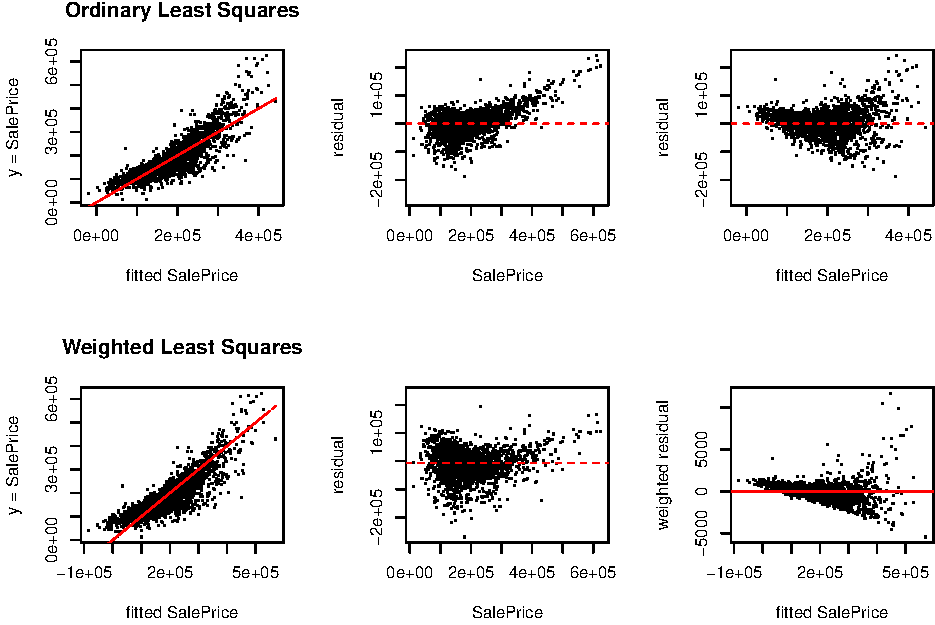
\includegraphics{./0_images/OLSvsWLS.pdf}
\caption{The top row panels represent the results for OLS linear regression, and the bottom row panels represent the results for WLS linear regression. The solid red represent fitted values (= $\widehat{y}$) of the housing prices (y = `SalePrice`). The dashed red lines represent the average of the (weighted) residuals (= $y - \widehat{y}$).}\label{fig:OLS_vs_WLS}
\end{figure}

In the case of the results for the OLS linear model, we see that the
residuals (= SalePrice - Fitted SalePrice) seem to become higher when
the prices (\texttt{SalePrice}) become higher. A too strong correlation
between the response (\texttt{SalePrice}) and the residuals is
undesirable, and is difficult to get rid off due to regulations provided
by a protocol of a certain mortgage provider. In this particular
protocol it states that\\
1. no transformation of the outcome variable is allowed;\\
2. nor a change in the formula of the linear model; and\\
3. a simple linear regression analysis has to be used (e.g.~using
\texttt{lm()} only).

Suppose a correct prediction of the higher prices is more lucrative (as
compared to the lower prices), then a solution is needed for this
specific linear model based on OLS. A solution could be to fit the
linear model based on weighted least squares (LM-WLS). With this
specific LM-WLS analysis you may find that you can assure that the
residuals are not (linearly) correlated with the actual housing prices,
see the middle panel on the bottom row of Figure \ref{fig:OLS_vs_WLS}.

Note that the linear model based on weighted least squares can still be
fitted with the function \texttt{lm()}. The only difference now is that
we use the argument \texttt{weights} in the function \texttt{lm()}.
Thus, we still comply with the protocol of the certain mortgage
provider.

\FloatBarrier 

\subsection{3.1 (5 points)}\label{points-3}

Fit and store the linear model with the formula \texttt{price\_model}
based on the ordinary least squares loss function on the prepared Ames
data.

Show that your object is very close or equal to linear model we used:
\texttt{lm\_ols} (see \texttt{Exam\_answer\_variables.RData}).

\subsection{\texorpdfstring{3.2 Recover the value for \(\lambda\) of the
WLS model (15
points)}{3.2 Recover the value for \textbackslash{}lambda of the WLS model (15 points)}}\label{recover-the-value-for-lambda-of-the-wls-model-15-points}

The linear model that we fitted based on WLS is stored in
\texttt{lm\_wls} (see \texttt{Exam\_answer\_variables.RData}). It was
fitted in the same way as the linear model based on OLS, but for the
\texttt{weights} argument we used the exponential weights of
\texttt{SalePrice} computed with a function based on equation
\eqref{eq:v_better}. Could you show with \texttt{R} code the value of
\(\lambda\) that we used?

The value for \(\lambda\) should be any of the values in

\begin{Shaded}
\begin{Highlighting}[]
\KeywordTok{as.numeric}\NormalTok{(}\KeywordTok{names}\NormalTok{(v_from_0_to_}\FloatTok{1e6}\NormalTok{))}
\end{Highlighting}
\end{Shaded}

\subsection{3.3 (10 points)}\label{points-4}

Replicate Figure \ref{fig:OLS_vs_WLS} by using either the results stored
in the variables \texttt{lm\_ols} and \texttt{lm\_wls}, or use your own
answers from subtasks 3.1 and 3.2.

\newpage

\section{4. About Bootstrapping for Validation (35
points).}\label{about-bootstrapping-for-validation-35-points.}

This exam's particular linear regression analysis based on WLS comes
with two disadvantages when compared to the OLS version: 1. it has a
higher Mean Squares Error; 2. it has a higher prediction error expressed
as \(1 - R^2\). Here, this prediction error can be expressed as

\begin{equation}
Err = 1 - COR(y, \widehat{y})^2,
\end{equation}

i.e.~where the squared Pearson correlation between the predicted outcome
\(\widehat{y}\) and the outcome variable \(y\) is substracted from 1.
Notet hat we have used this prediction error in one of the course weeks.

In this last task of the exam you will need to show that there is only a
very small increase in prediction error when using the WLS model, as
compared to the OLS model.

To do so, you will be programming a validation procedure that is
proposed as an improvement on cross-validation: The .632+ Bootstrap
Method (Efron \& Tibshirani, 1997).

\subsection{4.1. A probability of .632 (5
points)}\label{a-probability-of-.632-5-points}

It is a fact that bootstrap samples are supported on approximately
\(.632N\) of the original data points. When \(N\) is large enough, we
have \[\lim_{N \to \infty} P(i \in X^{b}) = 1 - e^{-1} \approx 0.632,\]
where \(X^{(b)}\) denotes a bootstrap sample and \(i\) an observation
that is present in the original sample \(X\).

Create a function that computes the exact probability that \(i\) ends up
(at least once) in the bootstrap sample \(X^{(b)}\), i.e.
\(P(i \in X^{b})\). Then, show in a visualization that this probability
already becomes \(\approx 1 - e^{-1}\) for \(N = 50\).

\emph{Hint: Compute \(1 - P(i \in X \in i \in X^{b})\). The probability
that an observation \(i\) is NOT the first observation in the bootstrap
sample is \(1 - 1/N\), and the sampling process is identical and
independent for all other observations in the boostrap sample.}

\subsection{4.2 A Smoothed Version of Cross-Validation: The .632+
Bootstrap Method (25
points)}\label{a-smoothed-version-of-cross-validation-the-.632-bootstrap-method-25-points}

For this subtask, write down the code for the resampling procedure that
is used inside the bootstrap method such that you can obtain an estimate
of the increase in prediction error. The algorithm can be programmed as
follows:

\subsubsection{The Algorithm}\label{the-algorithm}

Set \(B = 100\). Then, for each \(b \in \{1, \ldots, B\}\) bootstrap
samples of the data set \texttt{ames\_prep}, do the following:

\paragraph{\texorpdfstring{1. \textbf{Train the
models.}}{1. Train the models.}}\label{train-the-models.}

Let the bootstrap sample \(X^{b}\) be a training data set on which we
fit the linear model with OLS and the WLS linear regression model (as
was asked to you in subtaks 3.1 and 3.2.)

\paragraph{\texorpdfstring{2. \textbf{Training
error.}}{2. Training error.}}\label{training-error.}

Denote \(\widehat{y}^{(b)}_{OLS}\) and \(\widehat{y}^{(b)}_{WLS}\) as
the fitted values for \texttt{SalePrice} of the OLS and WLS models,
respectively. Define the increase in prediction error for your training
data set as

\begin{equation}
\overline{\text{err}}_b = cor({y}^{(b)}, \widehat{y}^{(b)}_{OLS})^2 - cor({y}^{(b)}, \widehat{y}^{(b)}_{WLS})^2,
\end{equation}

and store this specific value.

\paragraph{\texorpdfstring{3. \textbf{Obtain predictions for test
data.}}{3. Obtain predictions for test data.}}\label{obtain-predictions-for-test-data.}

Use the observations that were NOT selected in your bootstrap sample
\(X^{b}\) as the test data: \(X^{(-b)}\). Based on your trained OLS and
WLS models, obtain the predictions for the housing prices of the remain
objects denoted as \(\widehat{y}^{(-b)}_{OLS}\) and
\(\widehat{y}^{(-b)}_{WLS}\) respectively.

\paragraph{\texorpdfstring{4. \textbf{Test
error.}}{4. Test error.}}\label{test-error.}

Store the test error that can be computed as

\begin{equation}
\widehat{\text{Err}}^{(1)}_{b} = cor({y}^{(-b)} , \widehat{y}^{(-b)}_{OLS})^2 - cor({y}^{(-b)}, \widehat{y}^{(-b)}_{WLS})^2,
\end{equation}

After completing these for steps for each bootstrap sample, compute the
final increased training error as

\begin{equation}
\overline{\text{err}} = B^{-1} \sum^B_{b = 1} \overline{\text{err}}_b
\end{equation}

and the final increased test error as

\begin{equation}
\widehat{\text{Err}}^{(1)} = B^{-1} \sum^B_{b = 1} \widehat{\text{Err}}^{(1)}_{b}
\end{equation}

\emph{Hint 1: Decide for yourself how to deal with the exponential
weights in the WLS-model. Although not completely correct, when you also
bootstrap the exponential weights you can still obtain a perfect score
for this task.}

\emph{Hint 2: When you did not succeed in subtasks 3.1 and 3.2, then
either create this resampling procedure for a model and a prediction
error definition of your own choice, or use the \texttt{trained\_vars}
variable that is a list that contains of B lists for each bootstrap
sample. Each list of a bootstrap sample is again a list that contains
the in-sample indices of the observations, the OLS model results, and
the WLS model results.}

\subsection{4.3}\label{section}

To obtain a `good' estimate of the increase in prediction error, denoted
by \(\widehat{\text{Err}}^{(.632+)}\), Efron \& Tibshirani (1997) advise
to combine \(\overline{\text{err}}\) and \(\widehat{\text{Err}}^{(1)}\)
as follows:

\begin{equation}
\widehat{\text{Err}}^{(.632+)} = (1 - \widehat{w}) \overline{\text{err}}  +  \widehat{w} \widehat{\text{Err}}^{(1)}, 
\end{equation}

where \[ \widehat{w} = \frac{0.632}{1 - 0.368 \widehat{\text{ROR}}},\]
and \(0 \leq \widehat{\text{ROR}} \leq 1\) stands for the relative
overfitting rate. When \(\widehat{\text{ROR}} = 0\), then there is
basically no overfitting in the training error, and when
\(\widehat{\text{ROR}} = 1\) then there is a maximal amount of
overfitting.

To avoid that this exam becomes too long, let us assume that there is no
overfitting involved in the training error, i.e.
\(\widehat{\text{ROR}} = 0\).

What is the value of \(\widehat{\text{Err}}^{(.632+)}\)?

\emph{Hint: You can use \texttt{err\_bar} and \texttt{Err1} that came
with the answer variables in \texttt{Exam\_answer\_variables.RData}.}


\end{document}
